% Created 2016-12-02 Fri 09:22
\documentclass[t,10pt]{beamer}
\usepackage[utf8]{inputenc}
\usepackage[T1]{fontenc}
\usepackage{fixltx2e}
\usepackage{graphicx}
\usepackage{grffile}
\usepackage{longtable}
\usepackage{wrapfig}
\usepackage{rotating}
\usepackage[normalem]{ulem}
\usepackage{amsmath}
\usepackage{textcomp}
\usepackage{amssymb}
\usepackage{capt-of}
\usepackage{hyperref}
\mode<beamer>{\usetheme{Madrid}}
\hypersetup{colorlinks=true, linkcolor=blue}
\AtBeginSection[]{\begin{frame}<beamer>\frametitle{Topic}\tableofcontents[currentsection]\end{frame}}
\usetheme{Madrid}
\author{Stephen A. Sefick}
\date{2016-12-02}
\title{The Biogeography of Speciation: new genomic insights about reinforcement using biological collections}

\hypersetup{
 pdfauthor={Stephen A. Sefick},
 pdftitle={The Biogeography of Speciation: new genomic insights about reinforcement using biological collections},
 pdfkeywords={},
 pdfsubject={},
 pdfcreator={Emacs 24.3.1 (Org mode 8.3.6)}, 
 pdflang={English}}
\begin{document}

\maketitle
\begin{frame}{Outline}
\tableofcontents
\end{frame}



\section{Introduction}
\label{sec:orgheadline32}
\begin{frame}[<+->][label={sec:orgheadline1}]{Motivation}
\begin{enumerate}
\item Speciation
\begin{itemize}
\item Speciation results in biodiversity
\item Biodiversity declining
\item \alert{Important to study how biodiversity is produced} \vspace{0.25in}
\end{itemize}
\item Biogeography important to speciation process \vspace{0.25in}
\item Genomics
\begin{itemize}
\item since 2006 near exponential increase in genomic data
\item Recently computationaly feasable to identify genetic variants 
\begin{itemize}
\item simple
\item complex \vspace{0.25in}
\end{itemize}
\end{itemize}
\item \alert{Transform our understanding of the relationship of biogeography with speciation}
\end{enumerate}
\end{frame}

\begin{frame}[label={sec:orgheadline2}]{Types of speciation}
\end{frame}
\begin{frame}[label={sec:orgheadline3}]{Types of speciation}
\begin{enumerate}[<+->]
\item Allopatric Speciation
\begin{itemize}
\item interupted species range (i.e., stream)
\item decreased migration and gene flow
\item 2 incipient species \vspace{0.25in}
\end{itemize}
\end{enumerate}
\end{frame}


\begin{frame}[label={sec:orgheadline4}]{Allopatric Speciation}
\begin{figure}[htb]
\centering

\includegraphics[width=3in,height=3in]{./Figures/Allopatric_Speciation_Figure/png/1_Allopatric_Speciation.png}
\end{figure}
\end{frame}
\begin{frame}[label={sec:orgheadline5}]{Allopatric Speciation}
\begin{figure}[htb]
\centering
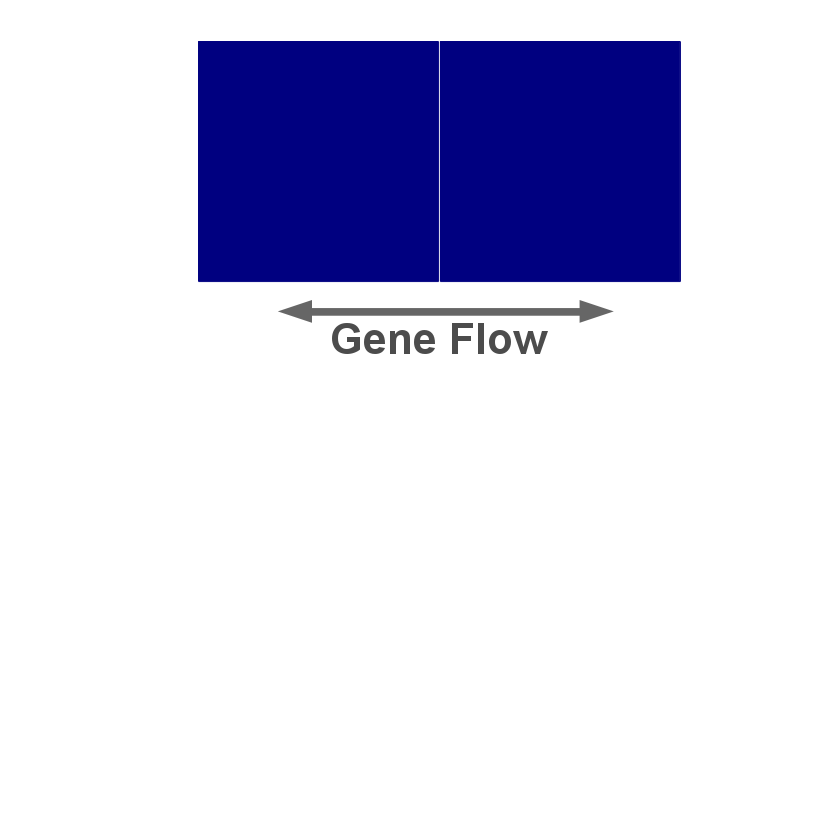
\includegraphics[width=3in,height=3in]{./Figures/Allopatric_Speciation_Figure/png/2_Allopatric_Speciation.png}
\end{figure}
\end{frame}
\begin{frame}[label={sec:orgheadline6}]{Allopatric Speciation}
\begin{figure}[htb]
\centering
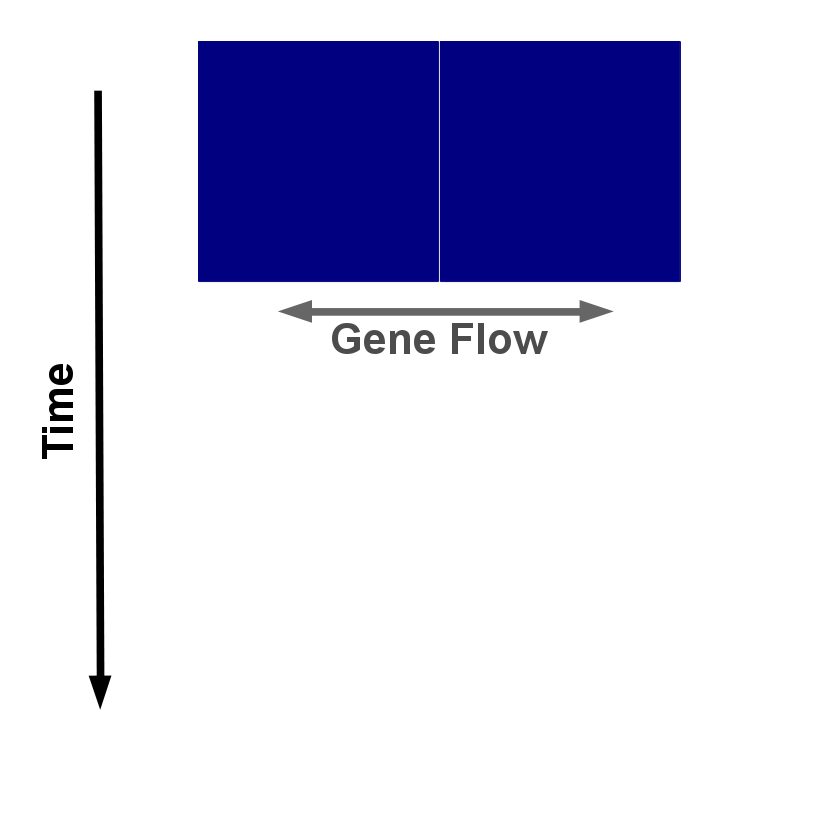
\includegraphics[width=3in,height=3in]{./Figures/Allopatric_Speciation_Figure/png/3_Allopatric_Speciation.png}
\end{figure}
\end{frame}
\begin{frame}[label={sec:orgheadline7}]{Allopatric Speciation}
\begin{figure}[htb]
\centering
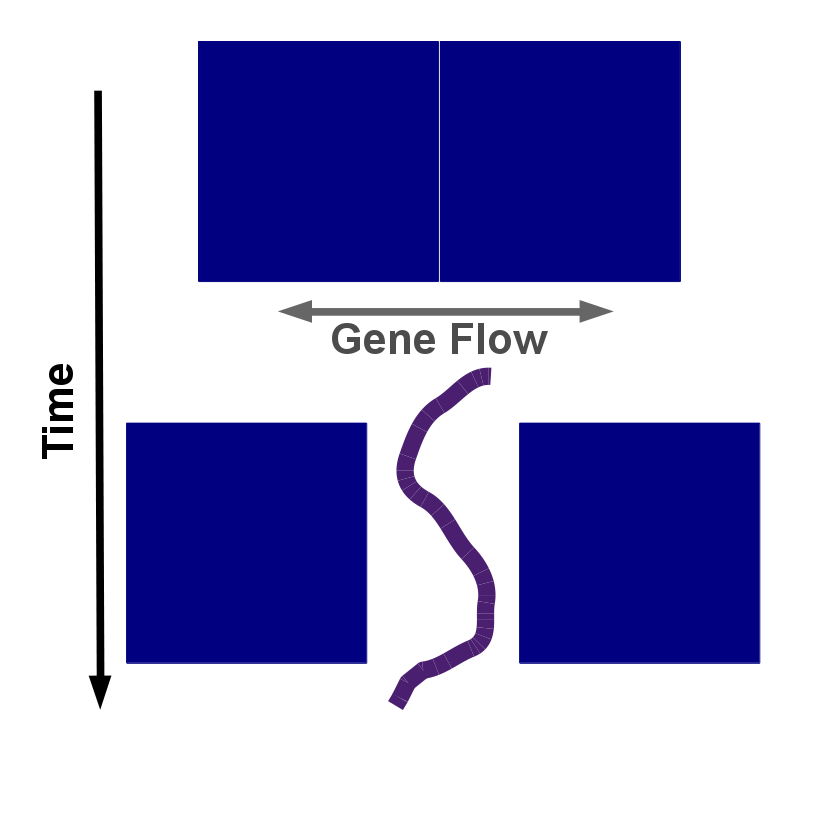
\includegraphics[width=3in,height=3in]{./Figures/Allopatric_Speciation_Figure/png/4_Allopatric_Speciation.png}
\end{figure}
\end{frame}
\begin{frame}[label={sec:orgheadline8}]{Allopatric Speciation}
\begin{figure}[htb]
\centering
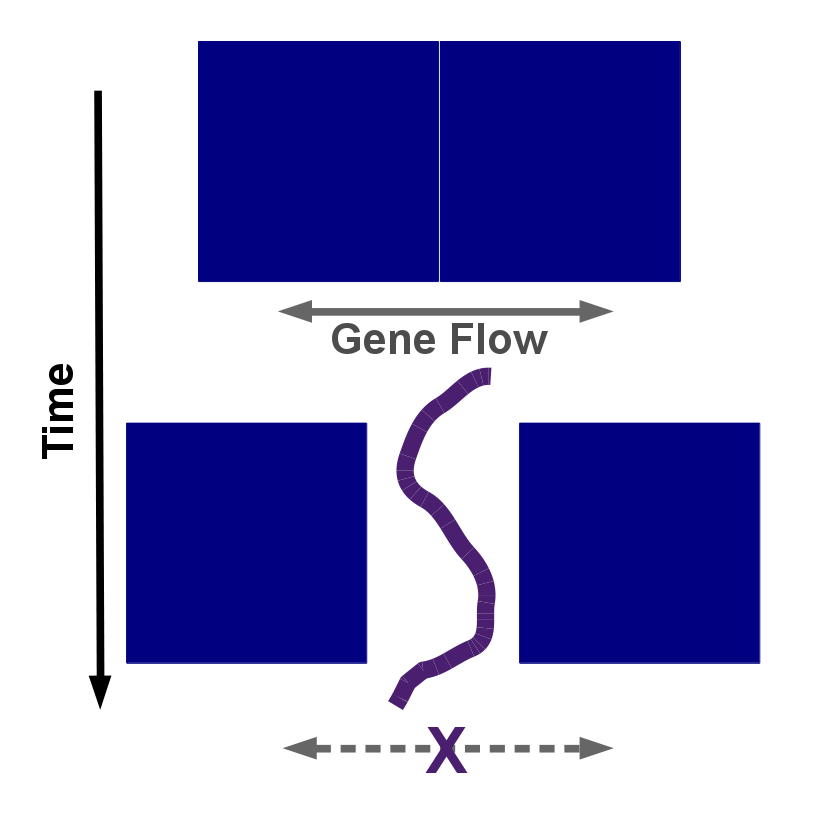
\includegraphics[width=3in,height=3in]{./Figures/Allopatric_Speciation_Figure/png/5_Allopatric_Speciation.png}
\end{figure}
\end{frame}
\begin{frame}[label={sec:orgheadline9}]{Allopatric Speciation}
\begin{figure}[htb]
\centering
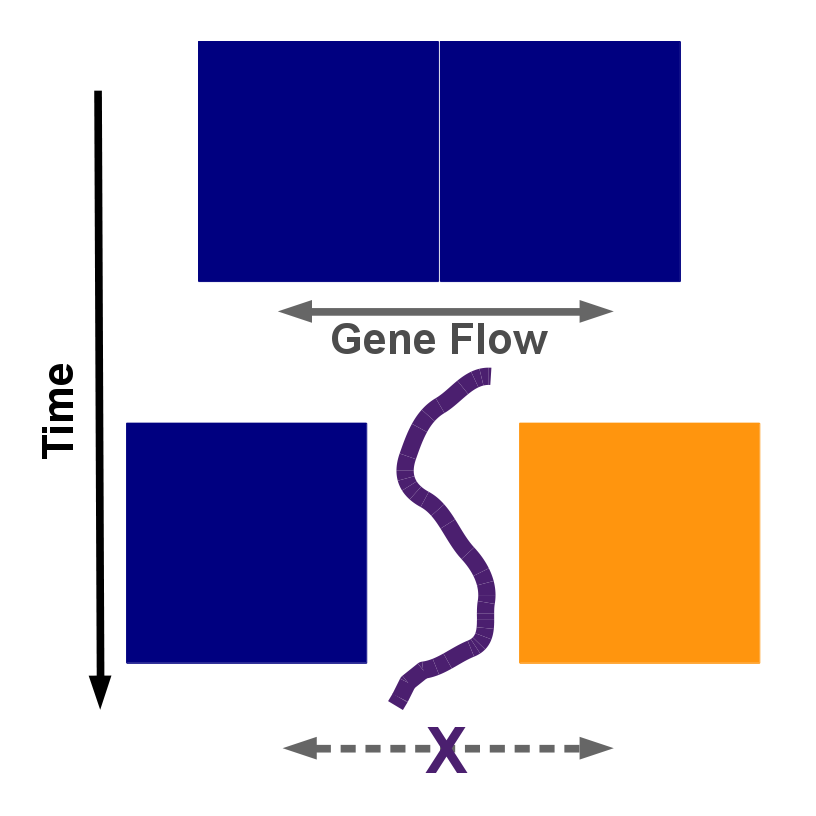
\includegraphics[width=3in,height=3in]{./Figures/Allopatric_Speciation_Figure/png/6_Allopatric_Speciation.png}
\end{figure}
\end{frame}

\begin{frame}[label={sec:orgheadline10}]{Types of speciation}
2 main types of speciation in a biogeographic context
\begin{enumerate}
\item Allopatric Speciation
\begin{itemize}
\item interupted species range (i.e., stream)
\item decreased migration and gene flow
\item 2 incipient species \vspace{0.25in}
\end{itemize}
\end{enumerate}
\begin{enumerate}[<+->]
\item Sympatric Speciation
\begin{itemize}
\item no species range interuption
\item proceeds with gene flow
\item 2 incipient species \vspace{0.25in}
\end{itemize}
\end{enumerate}
\end{frame}


\begin{frame}[label={sec:orgheadline11}]{Sympatric Speciation}
\begin{figure}[htb]
\centering

\includegraphics[width=3in,height=3in]{./Figures/Sympatric_Speciation_Figure/png/1_Sympatric_Speciation.png}
\end{figure}
\end{frame}
\begin{frame}[label={sec:orgheadline12}]{Sympatric Speciation}
\begin{figure}[htb]
\centering
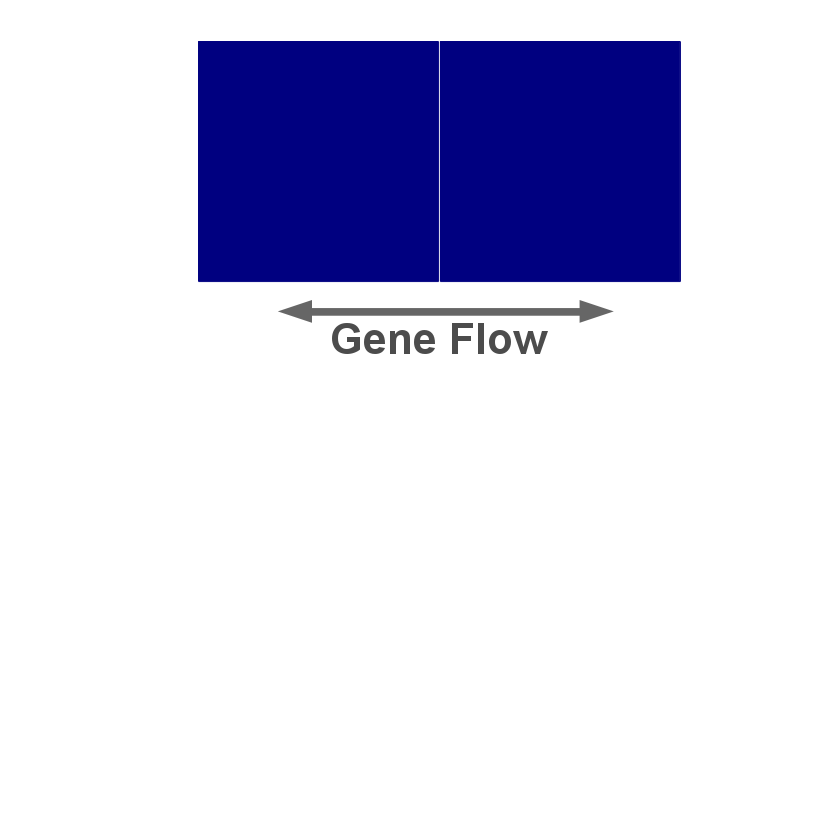
\includegraphics[width=3in,height=3in]{./Figures/Sympatric_Speciation_Figure/png/2_Sympatric_Speciation.png}
\end{figure}
\end{frame}
\begin{frame}[label={sec:orgheadline13}]{Sympatric Speciation}
\begin{figure}[htb]
\centering
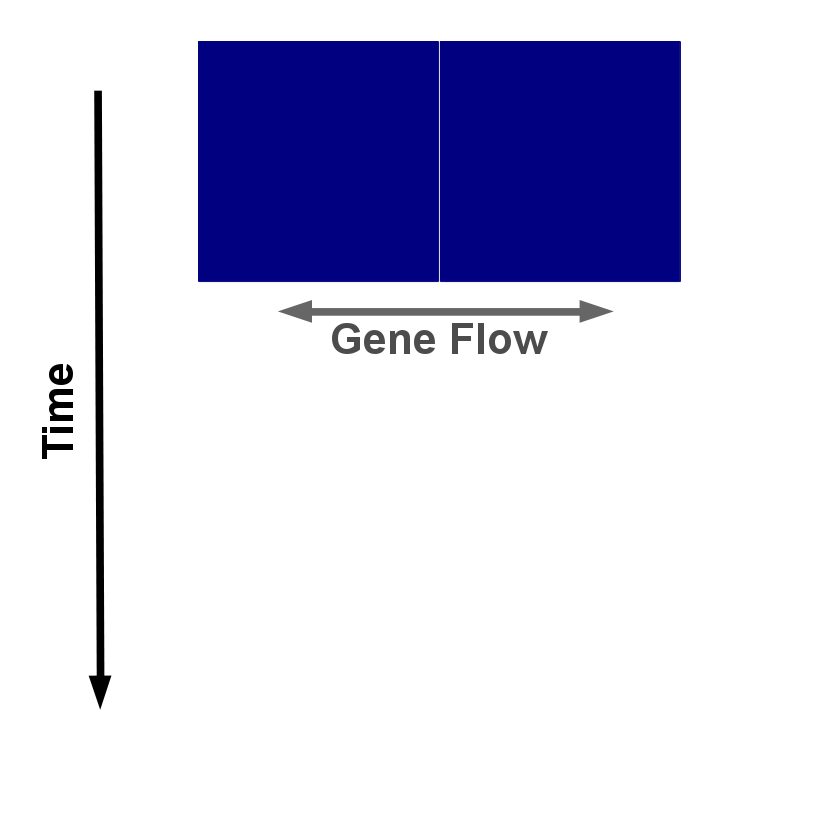
\includegraphics[width=3in,height=3in]{./Figures/Sympatric_Speciation_Figure/png/3_Sympatric_Speciation.png}
\end{figure}
\end{frame}
\begin{frame}[label={sec:orgheadline14}]{Sympatric Speciation}
\begin{figure}[htb]
\centering
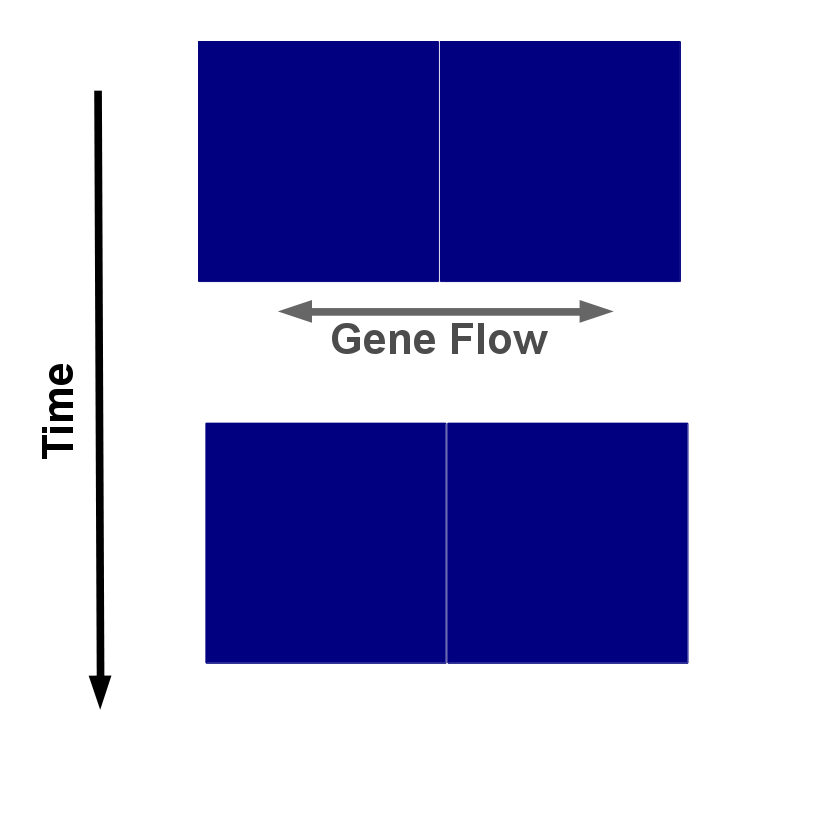
\includegraphics[width=3in,height=3in]{./Figures/Sympatric_Speciation_Figure/png/4_Sympatric_Speciation.png}
\end{figure}
\end{frame}
\begin{frame}[label={sec:orgheadline15}]{Sympatric Speciation}
\begin{figure}[htb]
\centering
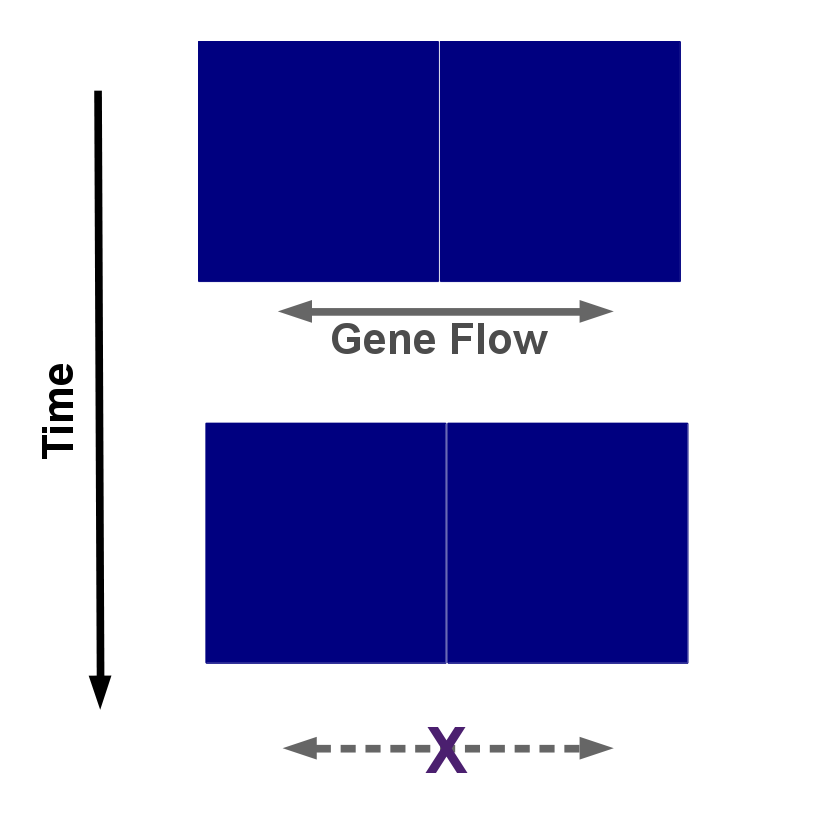
\includegraphics[width=3in,height=3in]{./Figures/Sympatric_Speciation_Figure/png/5_Sympatric_Speciation.png}
\end{figure}
\end{frame}
\begin{frame}[label={sec:orgheadline16}]{Sympatric Speciation}
\begin{figure}[htb]
\centering
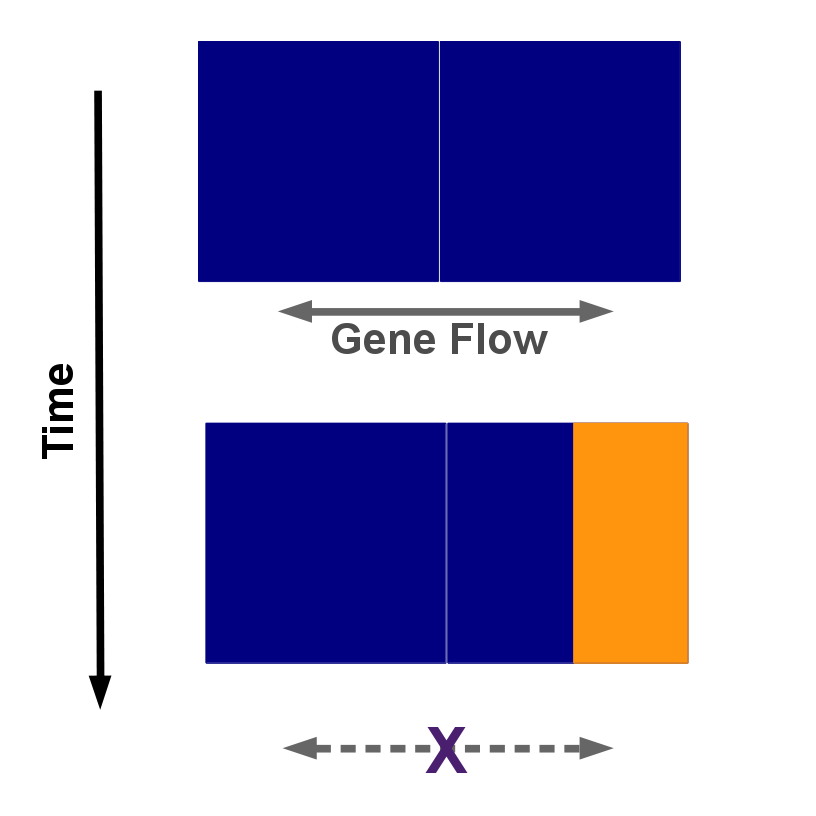
\includegraphics[width=3in,height=3in]{./Figures/Sympatric_Speciation_Figure/png/6_Sympatric_Speciation.png}
\end{figure}
\end{frame}


\begin{frame}[label={sec:orgheadline17}]{Types of speciation}
\begin{enumerate}
\item Allopatric Speciation
\begin{itemize}
\item interupted species range (i.e., stream)
\item decreased migration and gene flow
\item 2 incipient species \vspace{0.25in}
\end{itemize}
\item Sympatric Speciation
\begin{itemize}
\item no geographic interuption
\item proceeds with geneflow
\item 2 incipient species
\item<2-> \alert{Reinforcement recently shown to be important} \vspace{0.25in}
\end{itemize}
\end{enumerate}
\end{frame}

\begin{frame}[label={sec:orgheadline18}]{What is reinforcement?}
\end{frame}
\begin{frame}[<+->][label={sec:orgheadline19}]{What is reinforcement?}
\begin{enumerate}
\item 2 previously \alert{allopatric} populations come into contact
\item Speciation process not complete
\item There is selection against hybrids
\begin{itemize}
\item Reproductive character displacement
\end{itemize}
\end{enumerate}
\end{frame}


\begin{frame}[label={sec:orgheadline20}]{Flycatchers}
\begin{figure}[htb]
\centering
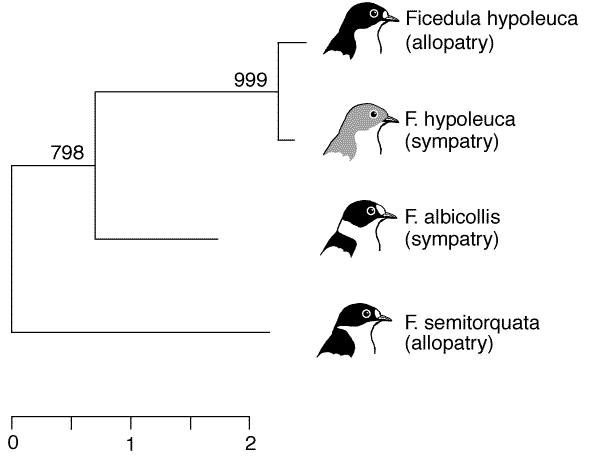
\includegraphics[width=3in,height=2.5in]{./Figures/FlycatcherPhylogeny.png}
Stre et al. 1997
\end{figure}
\end{frame}


\begin{frame}[label={sec:orgheadline21}]{What is reinforcement?}
\begin{enumerate}
\item 2 previously \alert{allopatric} populations come into contact
\item Speciation process not complete
\item There is selection against hybrids
\begin{itemize}
\item Reproductive character displacement
\item<2-> Ecological character displacement
\end{itemize}
\end{enumerate}
\end{frame}

\begin{frame}[label={sec:orgheadline22}]{Naked mole rat}
\begin{figure}[htb]
\centering
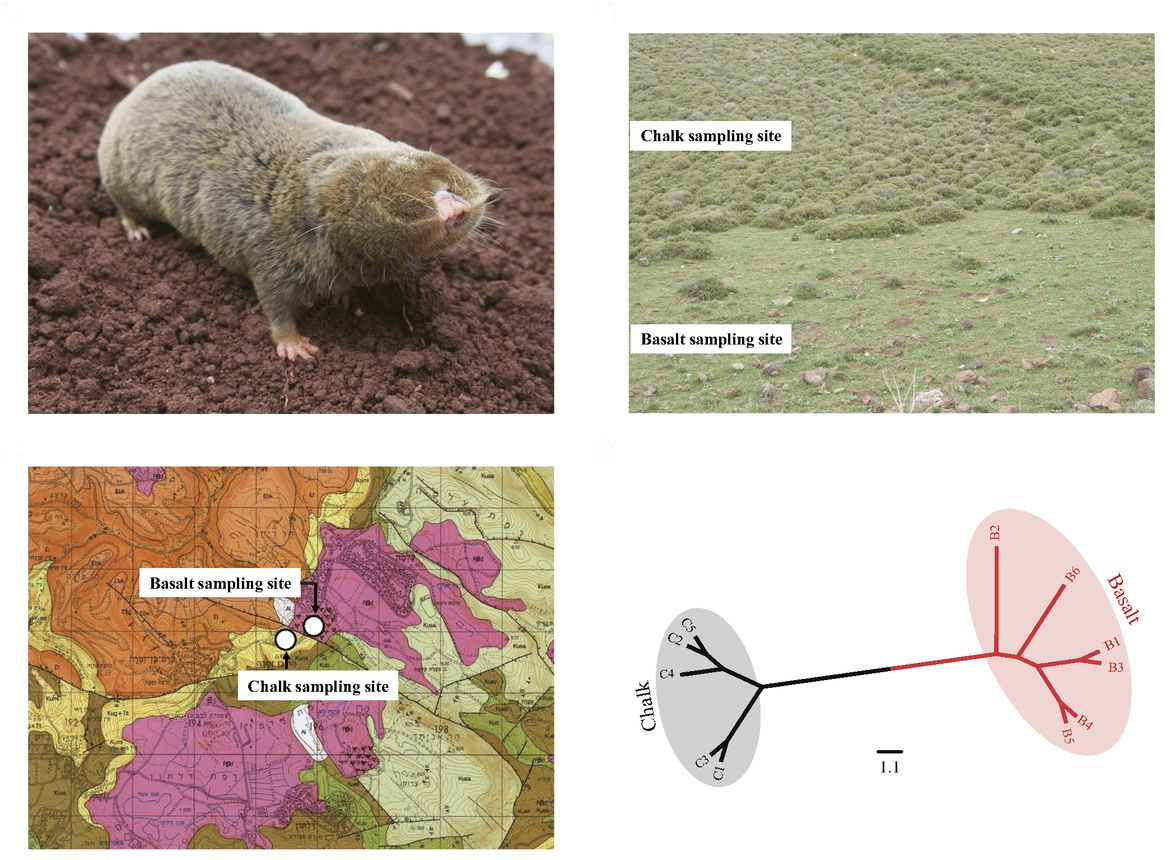
\includegraphics[width=3in,height=2.5in]{./Figures/naked_mole_rat.png}
Li et al. 2015
\end{figure}
\end{frame}

\begin{frame}[label={sec:orgheadline23}]{What is reinforcement?}
\begin{enumerate}
\item 2 previously \alert{allopatric} populations come into contact
\item Speciation process not complete
\item There is selection against hybrids
\begin{itemize}
\item Reproductive character displacement
\item Ecological character displacement
\end{itemize}
\item<2-> 2 incipient species result
\end{enumerate}
\end{frame}

\begin{frame}[label={sec:orgheadline24}]{Biogeographic and phylogenetic test for reinforcement}
\begin{figure}[htb]
\centering
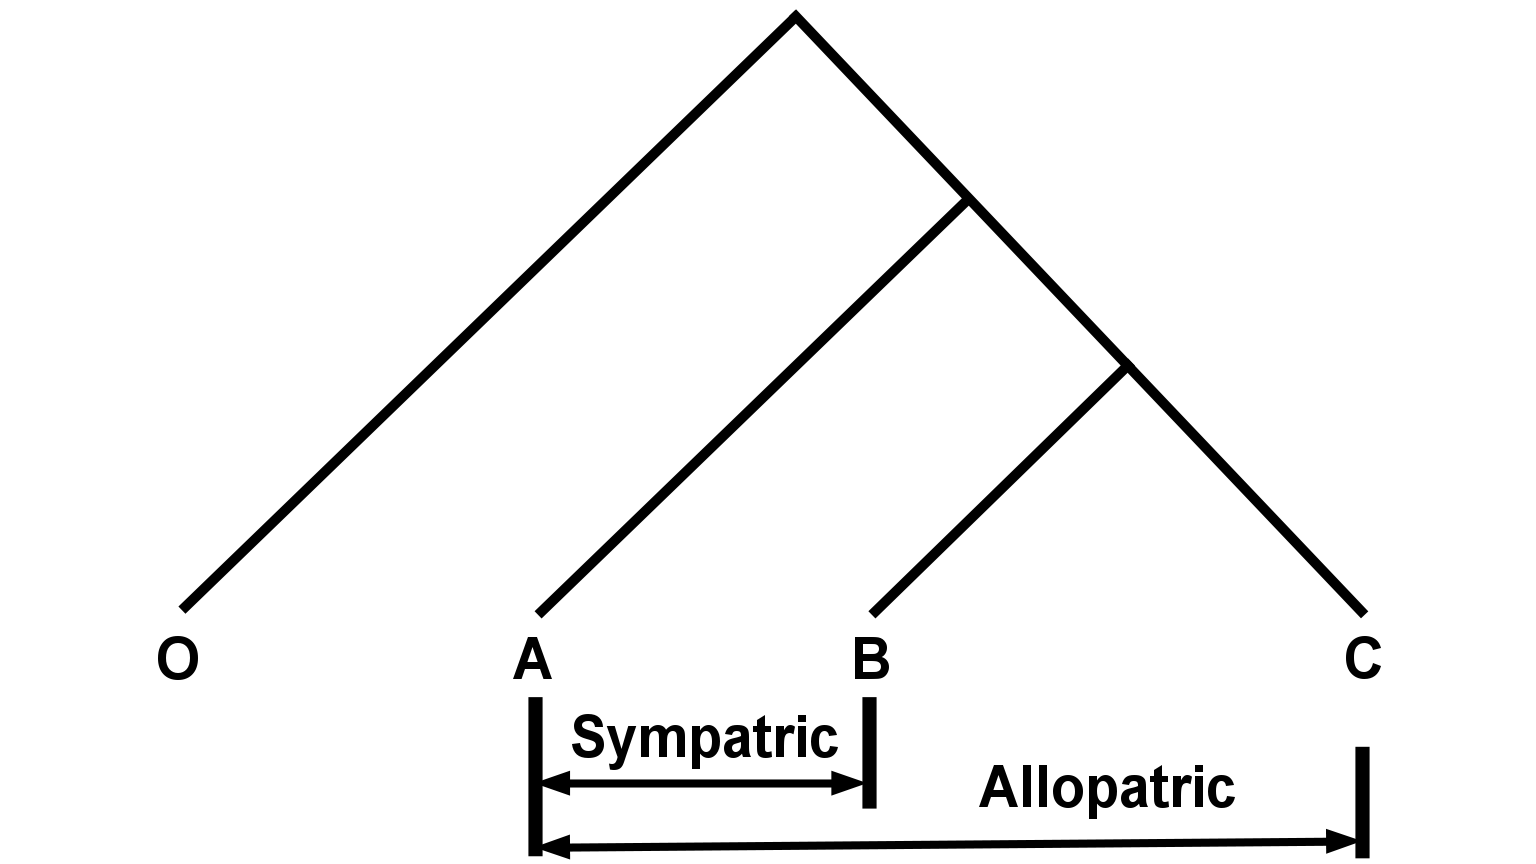
\includegraphics[width=3.5in,height=2.3in]{./Figures/Biogeography_of_Speciation_phylogeny.png}
Noor 1997
\end{figure}
\end{frame}

\begin{frame}[label={sec:orgheadline25}]{Biogeographic and phylogenetic test for reinforcement}
\begin{columns}
\begin{column}{0.5\columnwidth}
\begin{itemize}[<+->]
\item Species B more often different from A than C
\item Originally for reproductive isolation
\item Logic of test can be applied to genetic variants
\end{itemize}
\end{column}
\begin{column}{0.5\columnwidth}
\begin{figure}[htb]
\centering
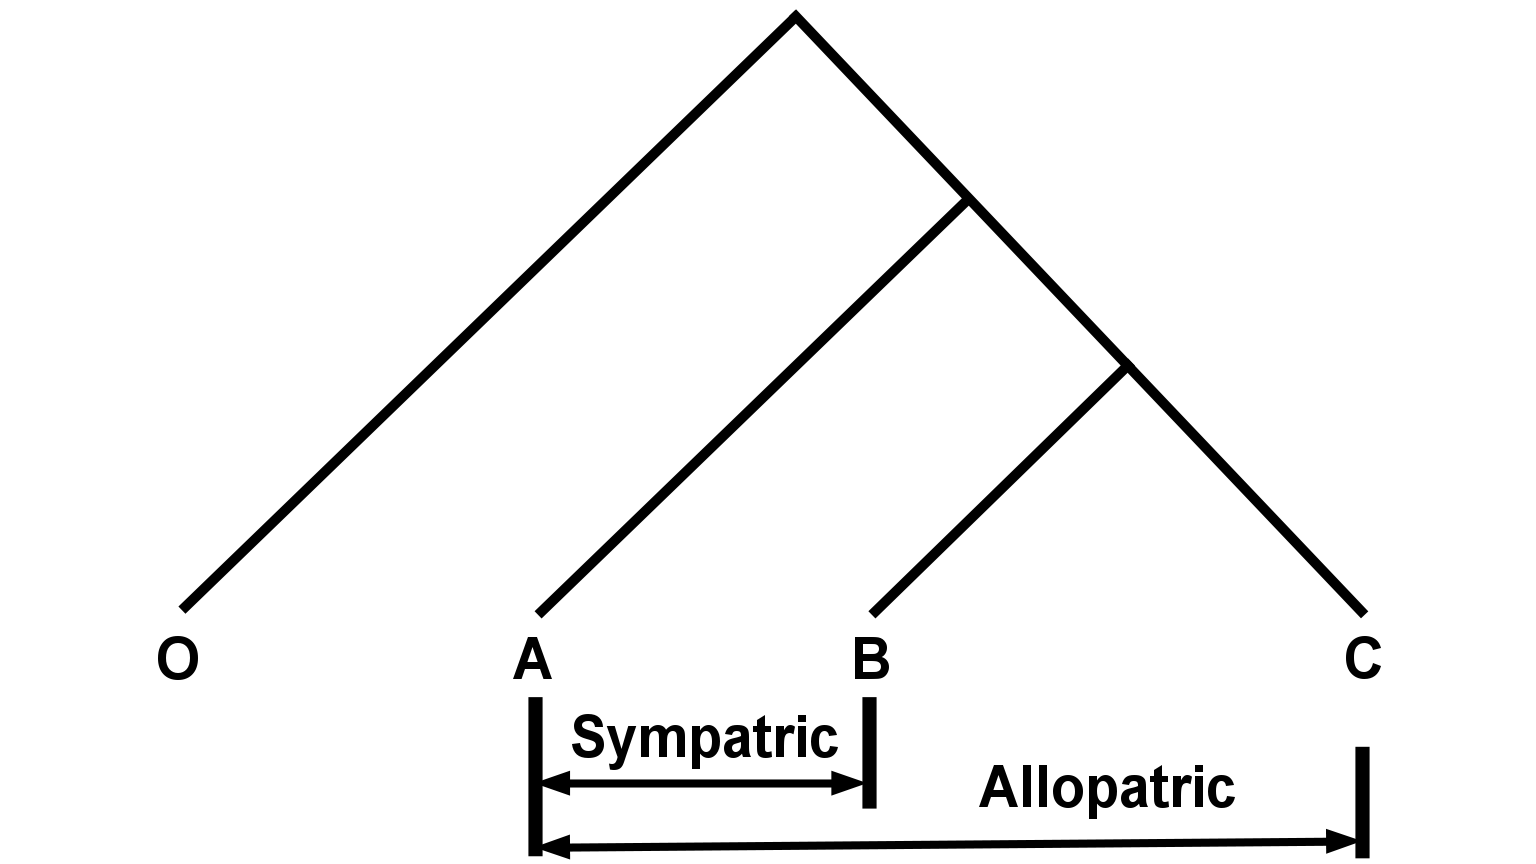
\includegraphics[width=2.5in,height=1.3in]{./Figures/Biogeography_of_Speciation_phylogeny.png}
\end{figure}
\end{column}
\end{columns}
\end{frame}


\begin{frame}[label={sec:orgheadline26}]{Genetic variants}
\begin{itemize}
\item What exactly are genetic variants?
\end{itemize}
\end{frame}
\begin{frame}[label={sec:orgheadline27}]{Genetic variants: Transposable elements}
\begin{figure}[htb]
\centering
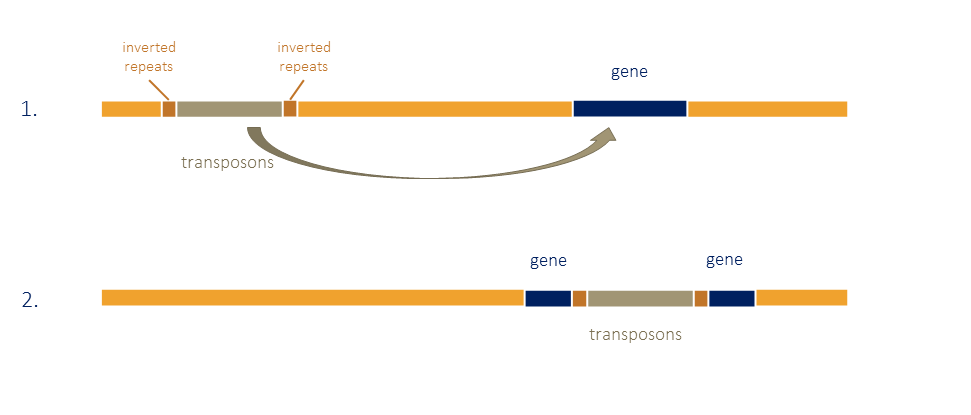
\includegraphics[width=2.5in,height=2.5in]{./Figures/Tranposons.png}
\end{figure}
\end{frame}

\begin{frame}[label={sec:orgheadline28}]{Genetic variants: Short tandem repeats}
\begin{figure}[htb]
\centering
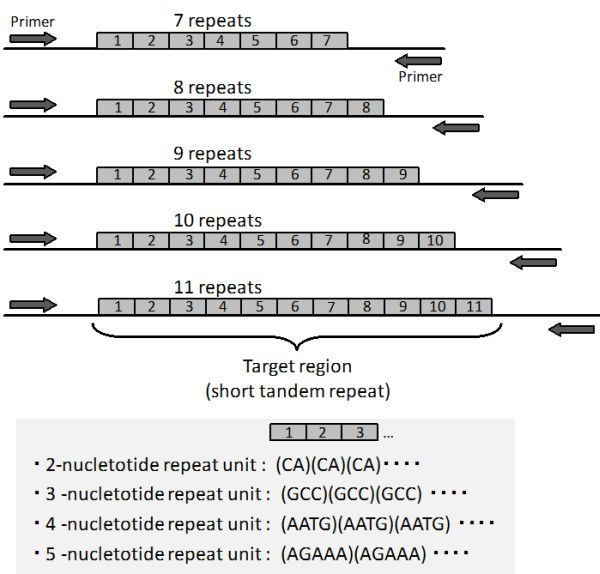
\includegraphics[width=2.5in,height=2.5in]{./Figures/STR.jpg}
\end{figure}
\end{frame}

\begin{frame}[label={sec:orgheadline29}]{Genetic variants: Structural Variants}
\begin{figure}[htb]
\centering
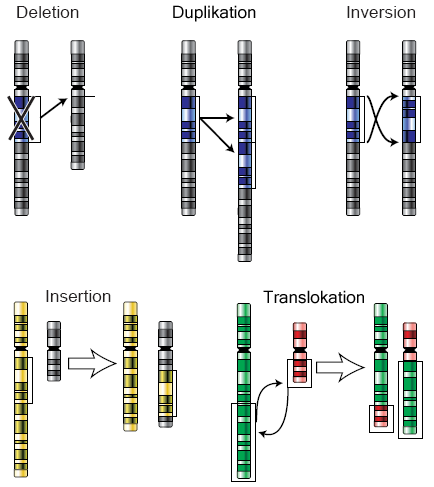
\includegraphics[width=2.5in,height=2.5in]{./Figures/Chromosomenmutationen.png}
\end{figure}
\end{frame}

\begin{frame}[label={sec:orgheadline30}]{Genetic variants: Single nucleotide polymorphisms}
\begin{figure}[htb]
\centering

\includegraphics[width=2.5in,height=2.5in]{./Figures/SNP.jpg}
\end{figure}
\end{frame}


\begin{frame}[<+->][label={sec:orgheadline31}]{Objectives and Hypotheses}
\begin{itemize}
\item Objective: Use a diverse set of taxa with genomic data in online biological collections to investigate the relationship of genetic variants with biogeography. \vspace{0.25in}

\item H1: Complex genomic variants will show the pattern of \alert{reinforcement}. \vspace{0.25in}

\item H2: SNPs representative of \alert{reinforcement} will be associated with functions indicative of ecological character displacement. \vspace{0.25in}
\end{itemize}
\end{frame}


\section{Methods}
\label{sec:orgheadline40}
\begin{frame}[label={sec:orgheadline33}]{Identify species groups}
\end{frame}
\begin{frame}[label={sec:orgheadline34}]{Identify species groups}
\begin{itemize}[<+->]
\item Conducted literature review
\begin{itemize}
\item phylogeny
\item biogeographic context
\item whole genome sequencing
\end{itemize}
\item Publically avaliable data (e.g., NCBI)
\end{itemize}
\end{frame}

\begin{frame}[label={sec:orgheadline35}]{Identify species groups}
\begin{itemize}
\item Conducted literature review
\begin{itemize}
\item phylogeny
\item biogeographic context
\item whole genome sequencing
\end{itemize}
\item Publically avaliable data (e.g., NCBI)
\item Appropriate phylogeny, biogeographic context, and whole genome sequencing
\end{itemize}
{\footnotesize
\begin{center}
\begin{tabular}{ll}
\hline
Organism & Acession Numbers\\
\hline
Mosquitoes (Anopheles) & NCBI: PRJNA6751 and PRJNA254046\\
Horses (Equus) & ENA: PRJEB7446\\
Butterflies (Heliconius) & ENA: ERP002440\\
Flycatchers (Ficula) & ENA: PRJEB7359\\
Dogs (Canis) & Authors Contacted\\
Cichlids & NCBI: PRJNA78915, PRJNA60369,PRJNA60363, and PRJNA78185\\
\hline
\end{tabular}
\end{center}
}
\end{frame}

\begin{frame}[label={sec:orgheadline36}]{Genetic Variants}
\begin{itemize}[<+->]
\item Download data (NCBI)
\item Use HPCs
\item GATK pipline (variant/variant filtration)
\begin{itemize}
\item SNPs
\end{itemize}
\item Computationionally identify complex genetic variants
\begin{itemize}
\item TEs
\item STRs
\item SVs
\end{itemize}
\end{itemize}
\end{frame}

\begin{frame}[label={sec:orgheadline37}]{Phylogenetic test for reinforcement}
\begin{columns}
\begin{column}{0.5\columnwidth}
\begin{itemize}[<+->]
\item Restrictions:
\begin{itemize}
\item C Allopatric to all other closely related species
\item but B and C some overlap 
\begin{itemize}
\item effects of sympatry shared
\end{itemize}
\end{itemize}
\item outgroup (O) to restrict search for genetic variants to those derived after most recent common ancestor
\item \[D=\frac{\sum_{n=1}^{i} Sym_{i}-Allo_{i}}{\sum_{n=1}^{i} Sym_{i}+Allo_{i}}\]
\item 1 > \emph{D} > -1
\begin{itemize}
\item Reinforcement \emph{D} > 0
\end{itemize}
\end{itemize}
\end{column}
\begin{column}{0.5\columnwidth}
\begin{figure}[htb]
\centering
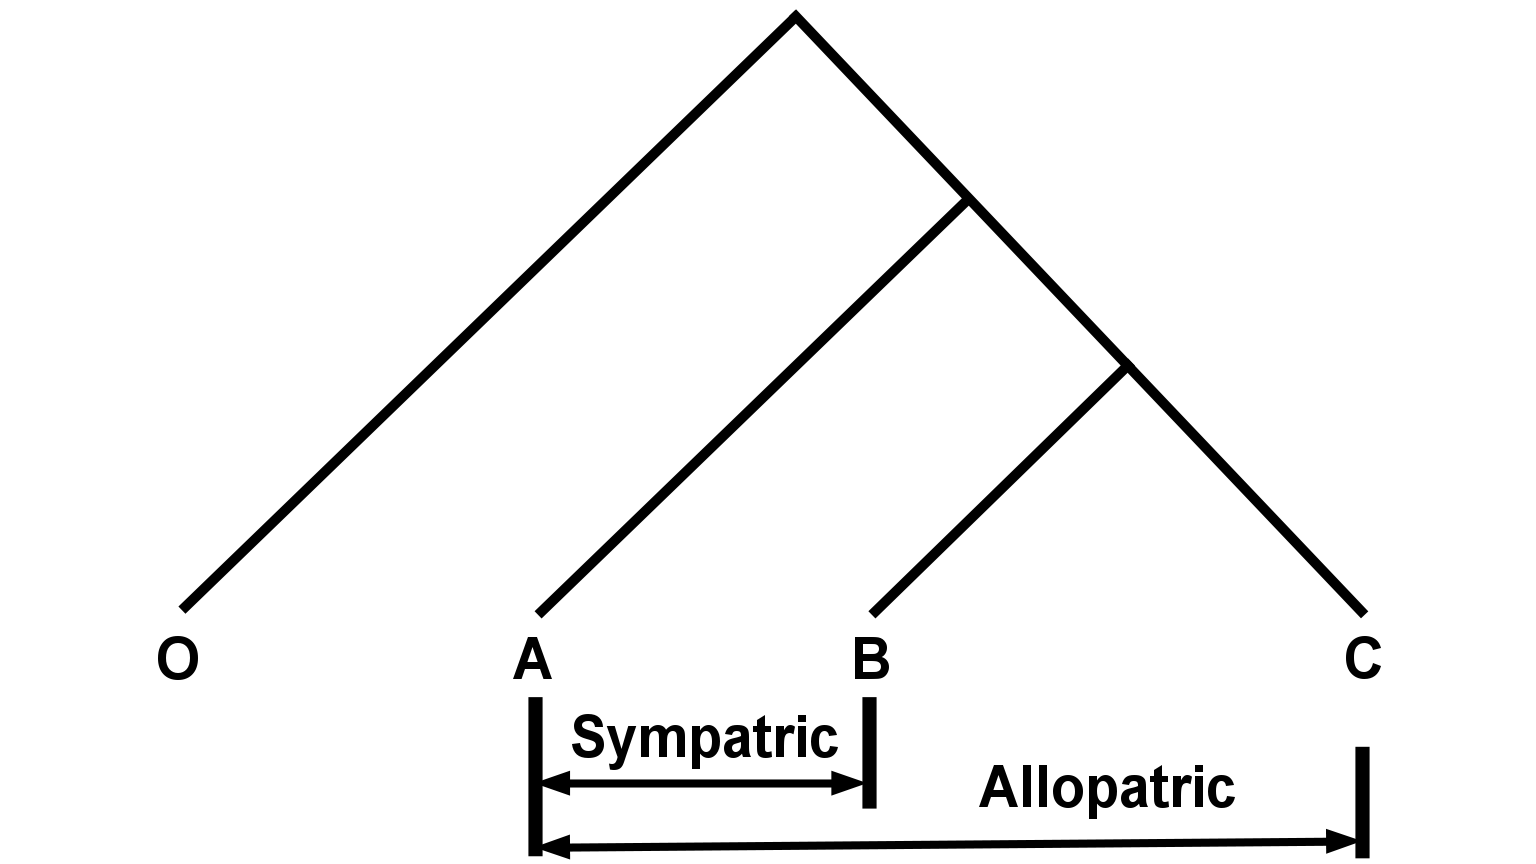
\includegraphics[width=2.5in,height=1.3in]{./Figures/Biogeography_of_Speciation_phylogeny.png}
\end{figure}
\end{column}
\end{columns}
\end{frame}
\begin{frame}[label={sec:orgheadline38}]{Reinforcement: Complex Genetic Variants}
\begin{itemize}[<+->]
\item H1: Complex genomic variants will show the pattern of \alert{reinforcement}. \vspace{0.25in}
\item Genome wide \emph{D}
\item Novel permutation proceedure to assess significance
\item Predictions
\begin{itemize}
\item Reinforcement \emph{D} > 0
\end{itemize}
\end{itemize}
\end{frame}

\begin{frame}[label={sec:orgheadline39}]{Reinforcement: Ecological Character Displacement}
\begin{itemize}[<+->]
\item H2: SNPs representative of \alert{reinforcement} will be associated with functions indicative of ecological character displacement. \vspace{0.25in}
\item \emph{D} in sliding windows
\item Novel permutation proceedure to assess significance
\item Use Gene Ontology to assign functions where \emph{D} > 0
\begin{itemize}
\item Use GO enrichment analysis
\end{itemize}
\item Predictions
\begin{itemize}
\item Significantly enriched GO terms ecological character displacement
\begin{itemize}
\item e.g., Habitat preferences
\end{itemize}
\end{itemize}
\item Alternatives
\begin{itemize}
\item Significantly enriched GO terms reproductive character displacement
\begin{itemize}
\item e.g., sperm development
\end{itemize}
\end{itemize}
\end{itemize}
\end{frame}
\section{Significance}
\label{sec:orgheadline42}
\begin{frame}[label={sec:orgheadline41}]{Significance}
\begin{itemize}[<+->]
\item taxonomic breadth \vspace{0.25in}
\item genetic variants (complex variants and SNPs) \vspace{0.25in}
\item Potential to transform our understanding of speciation's relationship with biogeography \vspace{0.25in}
\item Reveal impotant basic insights into how biodiversity is produced through speciation \vspace{0.25in}
\end{itemize}
\end{frame}

\section{Broader Impacts}
\label{sec:orgheadline44}
\begin{frame}[label={sec:orgheadline43}]{7th/8th Graders}
\begin{itemize}[<+->]
\item Speciation module AUMNH Junior Curator Camp
\item Computer Based Bioinformatics lesson
\item Program to connect online and traditional biological collections
\end{itemize}
\end{frame}
\section{Questions}
\label{sec:orgheadline46}
\begin{frame}[label={sec:orgheadline45}]{Questions}
\begin{figure}[htb]
\centering

\includegraphics[width=3in,height=3in]{./Figures/Bootsy.jpeg}
\end{figure}
\end{frame}
\end{document}
